\section{Representation and customer cluster structure}
\label{sec:paired-results}

This section answers RQ1 and RQ2 (\S\ref{sec:intro-rq}): how much do independently selected K Means and CLASSIX partitions agree across the two representations, and does that agreement coexist with high within-representation stability?

\textbf{Result.} Changing the represented information alters the selected customer structure for both clustering methods. Table~\ref{tab:customer_results} reports the independently selected deployment-acceptable configurations. K Means selects four clusters in each representation, but the agreement between the two four-cluster partitions is only 0.014 ARI. CLASSIX selects two compact clusters and three rich nonnoise clusters with 218 additional noise assignments (customers CLASSIX did not place in any final cluster, as defined in \S\ref{sec:classix-math}). Their cross-representation agreement is 0.068 ARI. Recall from \S\ref{sec:intro-content} that these ARI values compare the compact-space and rich-space partitions of the \emph{same} customers to each other, not to any external ground truth; both values are close to the score two unrelated random partitions of the same customers would obtain by chance, even though the customer identifiers and algorithm families are unchanged.

\begin{table}[htbp]
\centering
\caption{Deployment acceptable clustering results on the shared purchaser cohort. Noise records customers CLASSIX did not assign to any final cluster because no aggregation group containing them met the minimum-size or merging conditions to become one (\S\ref{sec:classix-math}); K Means never produces noise. Stability is mean fixed-parameter overlap-resampling ARI across ten resampled pairs (\S\ref{sec:resampling-explanation}).}
\label{tab:customer_results}
\begin{tabular}{llrrrrr}
\toprule
Representation & Method & Clusters & Noise & Largest share & Silhouette & Stability \\
\midrule
Compact & CLASSIX & 2 & 0 & 0.909 & 0.595 & 0.985 \\
Rich & CLASSIX & 3 & 218 & 0.898 & 0.291 & 0.965 \\
Compact & K Means & 4 & 0 & 0.664 & 0.560 & 0.988 \\
Rich & K Means & 4 & 0 & 0.579 & 0.351 & 0.995 \\
\bottomrule
\end{tabular}
\end{table}

\textbf{Mechanism.} \S\ref{sec:kmeans-math} and \S\ref{sec:classix-math} give the mechanical reason for this disagreement: both methods compute Euclidean distances (K Means directly; CLASSIX via its principal-direction projection) over \emph{all} standardised dimensions at once, so adding nine standardised behavioural dimensions changes every pairwise distance between customers, even though each customer's three original purchase coordinates are numerically unchanged. A different set of distances can move K Means's optimal centroids to different locations, and can change the covariance structure that determines CLASSIX's sorting direction — both of which can change the resulting partition without any change to the underlying customers.

The internal indices do not move in a single direction. Compact CLASSIX has silhouette 0.595, Davies Bouldin 1.057 and Calinski Harabasz 4285.5. The rich result has silhouette 0.291, Davies Bouldin 0.859 and Calinski Harabasz 1516.9. These CLASSIX values are calculated on each partition's nonnoise observations. Davies Bouldin favours the rich result, while silhouette and Calinski Harabasz favour the compact result. Compact K Means has silhouette 0.560 and Calinski Harabasz 10459.1, compared with 0.351 and 3923.4 in the rich space. Davies Bouldin rises from 0.775 to 1.040. Richer behaviour produces a different geometry whose apparent quality depends on the criterion.

\begin{figure}[htbp]
\centering
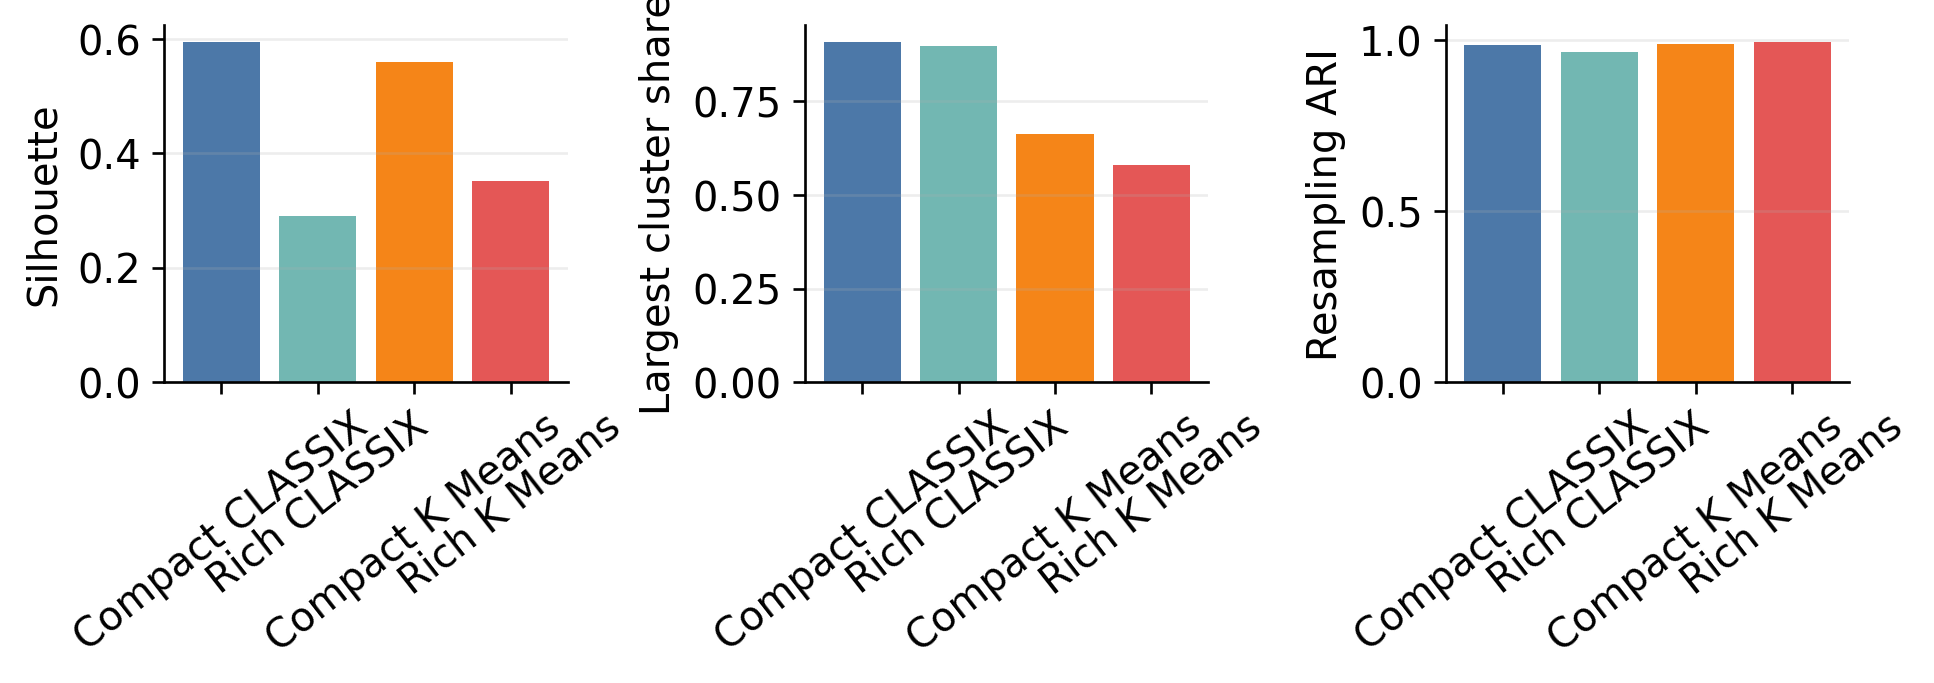
\includegraphics[width=0.80\textwidth]{figures/customer_structure.png}
\caption{Internal structure and resampling stability for the selected customer partitions}
\label{fig:customer_structure}
\end{figure}

The deployment rule materially changes the result that would be chosen by silhouette alone. Compact CLASSIX reaches silhouette 0.899 by placing 11,698 of 11,719 customers in one cluster. Rich CLASSIX reaches 0.792 with 11,716 customers in one cluster and the remaining three customers split across two tiny clusters. Compact K Means reaches 0.850 with 11,593 customers in one of two clusters. All three partitions fail the maximum share rule. The deployment selections sacrifice these high silhouette values to avoid reporting a nearly undivided customer base as a useful segmentation. Rich K Means is the only case where the unconstrained and deployment selections coincide.

Low agreement is not caused only by choosing different numbers of clusters. At every fixed K from 2 to 12, the K Means ARI between compact and rich representations remains between 0.012 and 0.113. At the common selected value of four it is 0.014, with NMI 0.089 and variation of information 1.691 nats. Under matched labels, 54.61 per cent of customers move to a different K Means cluster. Among 41 CLASSIX settings that are deployment acceptable in both spaces, matched-parameter ARI ranges from $-0.051$ to $0.392$ with a median of $-0.023$. The independently selected CLASSIX partitions have NMI 0.054 and variation of information 0.693 nats, with 18.66 per cent assigned to a different matched cluster or noise state. The lower CLASSIX migration share partly reflects the dominance of one large cluster in both representations and should not be read as stronger substantive agreement.

Cluster sizes make the changes more concrete. Compact K Means contains 7,784, 2,494, 1,344 and 97 customers. Rich K Means contains 6,790, 3,607, 1,156 and 166. Its 166 customer cluster has a median of 338.5 total events, 28 sessions and 12 top categories, whereas the full cohort medians are 6 events, 2 sessions and 1 top category. Another rich cluster of 1,156 customers has no known category at its median and a purchase recency median of 127.4 days. These are descriptive contrasts in observed features, not customer identities or causal segments.

CLASSIX yields a sharper imbalance. The compact deployment result contains 10,656 and 1,063 customers. The rich result contains 10,331, 1,137 and 33 nonnoise customers plus 218 noise assignments. The 33-customer cluster is highly active, with medians of 869 total events, 36 sessions and 14 top categories. Its small size fails the documented addressability size rule. The 1,137-customer cluster has zero category coverage and fails the coverage rule. The dominant 10,331-customer cluster has no two sufficiently distinctive median effects. Richer features expose unusual behavioural combinations, but the selected CLASSIX partition does not turn them into a balanced set of directly addressable clusters.

Fixed-parameter overlap-resampling indicates that these structural differences are reproducible under the stated sampling scheme. Mean overlap ARI is 0.985 for compact CLASSIX and 0.965 for rich CLASSIX. The corresponding K Means values are 0.988 and 0.995. The lowest of ten pairwise values is 0.881 for compact CLASSIX and 0.941 for rich CLASSIX.

\textbf{Interpretation.} This is the answer to RQ2: high within-representation stability and low cross-representation agreement are not contradictory, because they answer different questions. Stability (\S\ref{sec:resampling-explanation}) asks whether the \emph{same fixed recipe} reproduces a similar partition when refit on a slightly different 80 per cent of customers; cross-representation ARI asks whether \emph{two different recipes} (compact and rich) agree on the \emph{same} customers. A configuration can be highly self-consistent — reliably rediscovering its own partition under resampling — while still describing a genuinely different grouping from the other representation's equally self-consistent partition. This is direct evidence that representation is a modelling choice with its own reproducible consequences, not a preprocessing detail whose effect washes out once a method is "properly" fitted.

\textbf{Limitation.} Stable refitting does not imply that a partition is uniquely correct, that model \emph{selection} (choosing this configuration from the full grid in the first place) would recur under resampling, or that either partition would remain stable outside this cohort or over calendar time. It shows only that each selected representation and parameter combination tends to reproduce its own assignment pattern when one fifth of the cohort is omitted.
